\documentclass[11pt,a4paper]{report}
\usepackage[textwidth=37em,vmargin=30mm]{geometry}
\usepackage{calc,xunicode,amsmath,amssymb,paralist,enumitem,tabu,booktabs,datetime2,xeCJK,xeCJKfntef,listings}
\usepackage{tocloft,fancyhdr,tcolorbox,xcolor,graphicx,eso-pic,xltxtra,xelatexemoji}

\newcommand{\envyear}[0]{2025}
\newcommand{\envdatestr}[0]{2025-01-13}
\newcommand{\envfinaldir}[0]{webdb/2025/20250113/final}

\usepackage[hidelinks]{hyperref}
\hypersetup{
    colorlinks=false,
    pdfpagemode=FullScreen,
    pdftitle={Web Digest - \envdatestr}
}

\setlength{\cftbeforechapskip}{10pt}
\renewcommand{\cftchapfont}{\rmfamily\bfseries\large\raggedright}
\setlength{\cftbeforesecskip}{2pt}
\renewcommand{\cftsecfont}{\sffamily\small\raggedright}

\setdefaultleftmargin{2em}{2em}{1em}{1em}{1em}{1em}

\usepackage{xeCJK,xeCJKfntef}
\xeCJKsetup{PunctStyle=plain,RubberPunctSkip=false,CJKglue=\strut\hskip 0pt plus 0.1em minus 0.05em,CJKecglue=\strut\hskip 0.22em plus 0.2em}
\XeTeXlinebreaklocale "zh"
\XeTeXlinebreakskip = 0pt


\setmainfont{Brygada 1918}
\setromanfont{Brygada 1918}
\setsansfont{IBM Plex Sans}
\setmonofont{JetBrains Mono NL}
\setCJKmainfont{Noto Serif CJK SC}
\setCJKromanfont{Noto Serif CJK SC}
\setCJKsansfont{Noto Sans CJK SC}
\setCJKmonofont{Noto Sans CJK SC}

\setlength{\parindent}{0pt}
\setlength{\parskip}{8pt}
\linespread{1.15}

\lstset{
	basicstyle=\ttfamily\footnotesize,
	numbersep=5pt,
	backgroundcolor=\color{black!5},
	showspaces=false,
	showstringspaces=false,
	showtabs=false,
	tabsize=2,
	captionpos=b,
	breaklines=true,
	breakatwhitespace=true,
	breakautoindent=true,
	linewidth=\textwidth
}






\newcommand{\coverpic}[2]{
    % argv: itemurl, authorname
    Cover photo by #2~~(\href{#1}{#1})
}
\newcommand{\makeheader}[0]{
    \begin{titlepage}
        % \newgeometry{hmargin=15mm,tmargin=21mm,bmargin=12mm}
        \begin{center}
            
            \rmfamily\scshape
            \fontspec{BaskervilleF}
            \fontspec{Old Standard}
            \fontsize{59pt}{70pt}\selectfont
            WEB\hfill DIGEST
            
            \vfill
            % \vskip 30pt
            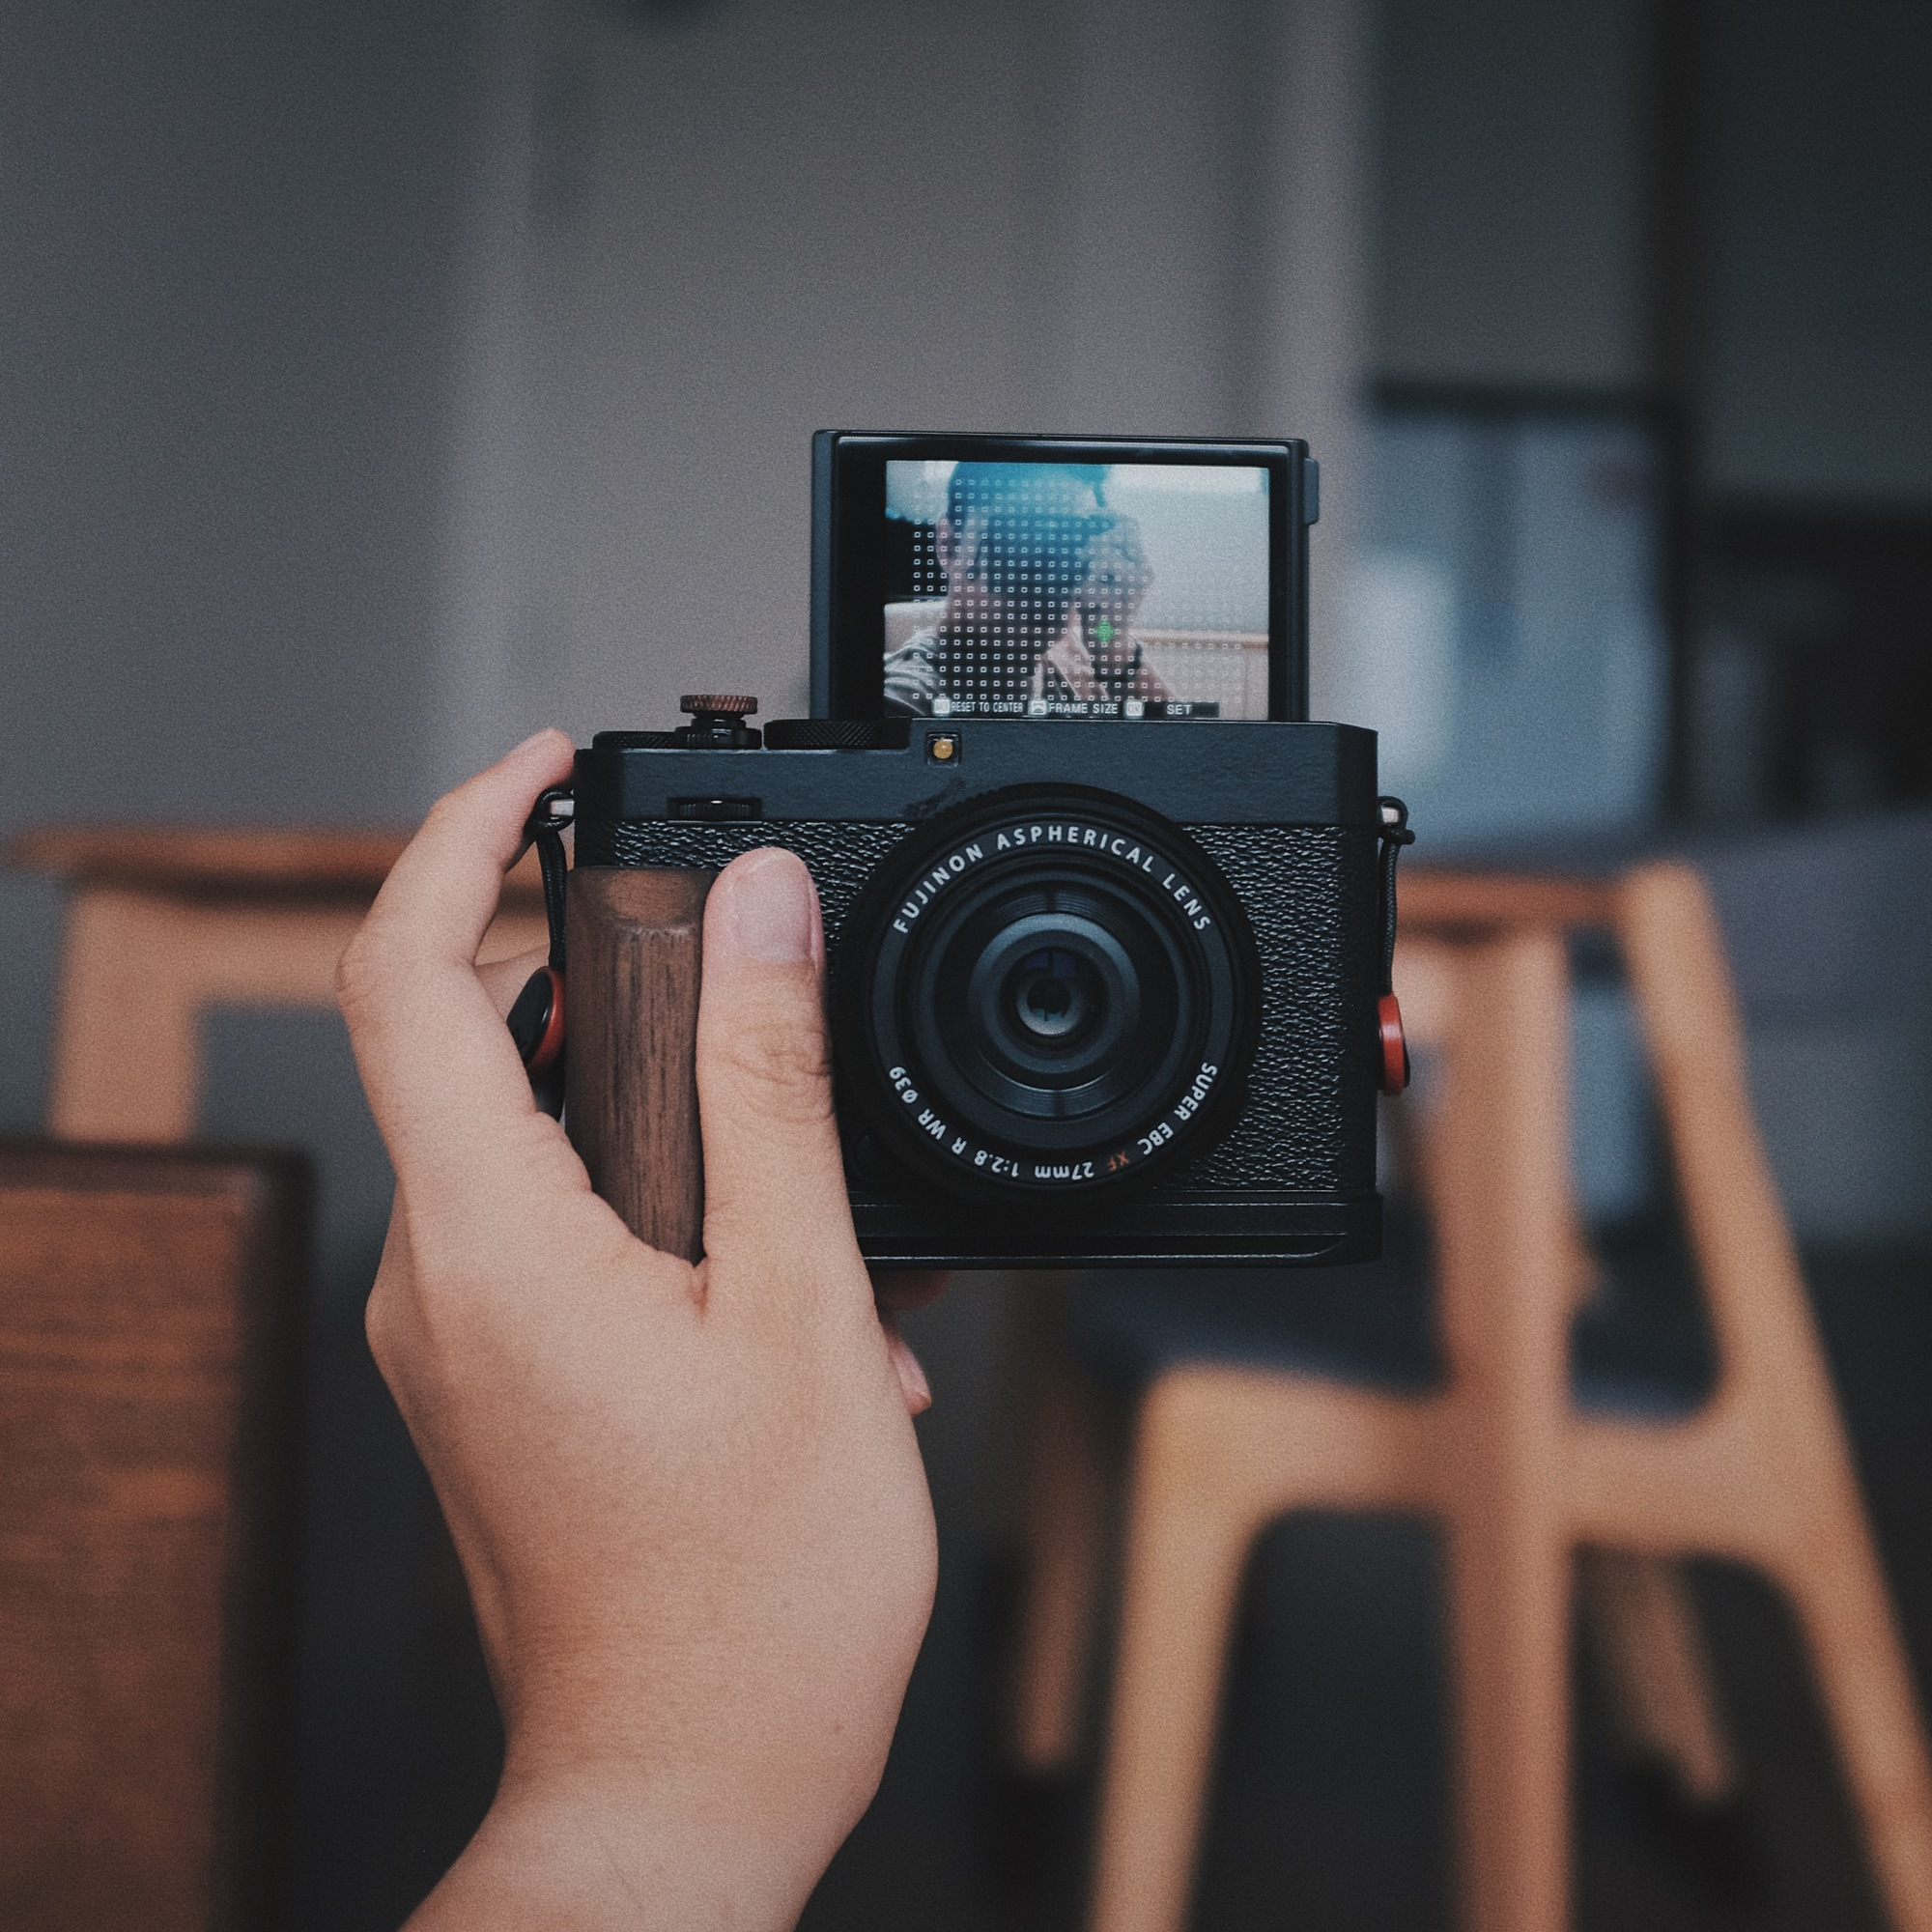
\includegraphics[width=\linewidth]{\envfinaldir/coverpic-prod.jpg}\par
            % \vskip 30pt
            \vfill

            \normalsize\rmfamily\scshape
            \copyright{} The Web Digest Project \hfill\large \envdatestr
        \end{center}
    \end{titlepage}
    % \restoregeometry
}
\newcommand{\simplehref}[1]{%
    \textcolor{blue!80!green}{\href{#1}{#1}}%
}
\renewcommand{\contentsname}{\center\Huge\sffamily\bfseries Contents\par\vskip 20pt}
\newcounter{ipartcounter}
\setcounter{ipartcounter}{0}
\newcommand{\ipart}[1]{
    % \vskip 20pt
    \clearpage
    \stepcounter{ipartcounter}
    \phantomsection
    \addcontentsline{toc}{chapter}{#1}
    % \begin{center}
    %     \Huge
    %     \sffamily\bfseries
    %     #1
    % \end{center}
    % \vskip 20pt plus 7pt
}
\newcounter{ichaptercounter}
\setcounter{ichaptercounter}{0}
\newcommand{\ichapter}[1]{
    % \vskip 20pt
    \clearpage
    \stepcounter{ichaptercounter}
    \phantomsection
    \addcontentsline{toc}{section}{\numberline{\arabic{ichaptercounter}}#1}
    \begin{center}
        \Huge
        \sffamily\bfseries
        #1
    \end{center}
    \vskip 20pt plus 7pt
}
\newcommand{\entrytitlefont}[1]{\subsection*{\raggedright\Large\sffamily\bfseries#1}}
\newcommand{\entryitemGeneric}[2]{
    % argv: title, url
    \parbox{\linewidth}{
        \entrytitlefont{#1}\par\vskip 5pt
        \footnotesize\ttfamily\mdseries
        \simplehref{#2}
    }\vskip 11pt plus 11pt minus 1pt
}
\newcommand{\entryitemGithub}[3]{
    % argv: title, url, desc
    \parbox{\linewidth}{
        \entrytitlefont{#1}\par\vskip 5pt
        \footnotesize\ttfamily\mdseries
        \simplehref{#2}\par\vskip 5pt
        \small\rmfamily\mdseries#3
    }\vskip 11pt plus 11pt minus 1pt
}
\newcommand{\entryitemAp}[3]{
    % argv: title, url, desc
    \parbox{\linewidth}{
        \entrytitlefont{#1}\par\vskip 5pt
        \footnotesize\ttfamily\mdseries
        \simplehref{#2}\par\vskip 5pt
        \small\rmfamily\mdseries#3
    }\vskip 11pt plus 11pt minus 1pt
}
\newcommand{\entryitemHackernews}[3]{
    % argv: title, hnurl, rawurl
    % \parbox{\linewidth}{
    %     \entrytitlefont{#1}\par\vskip 5pt
    %     \footnotesize\ttfamily\mdseries
    %     \simplehref{#3}\par
    %     \textcolor{black!50}{\href{#2}{#2}}
    % }\vskip 11pt plus 11pt minus 1pt
    \begin{minipage}{\linewidth}
            \entrytitlefont{#1}\par\vskip 5pt
            \footnotesize\ttfamily\mdseries
            \simplehref{#3}\par
            \textcolor{black!50}{\href{#2}{#2}}
    \end{minipage}\par\vskip 11pt plus 11pt minus 1pt
}







\begin{document}

\makeheader

\tableofcontents\clearpage




\ipart{Developers}
\ichapter{Hacker News}
\entryitemTwoLinks{I deleted my social media accounts (and why you should too)}{https://news.ycombinator.com/item?id=42677587}{https://asylumsquare.com/backstage/2025-01-12/why-i-deleted-my-social-media-accounts}

\entryitemTwoLinks{Uv's killer feature is pulling in local dependencies}{https://news.ycombinator.com/item?id=42676432}{https://valatka.dev/2025/01/12/on-killer-uv-feature.html}

\entryitemTwoLinks{Best Pens for 2025}{https://news.ycombinator.com/item?id=42676274}{https://www.jetpens.com/blog/The-46-Best-Pens-for-2025-Gel-Ballpoint-Rollerball-and-Fountain-Pens/pt/974}

\entryitemTwoLinks{Tabby: Self-hosted AI coding assistant}{https://news.ycombinator.com/item?id=42675725}{https://github.com/TabbyML/tabby}

\entryitemTwoLinks{The Case for Letting Malibu Burn (1995)}{https://news.ycombinator.com/item?id=42675274}{https://longreads.com/2018/12/04/the-case-for-letting-malibu-burn/}

\entryitemTwoLinks{Great things about Rust that aren't just performance}{https://news.ycombinator.com/item?id=42675219}{https://ntietz.com/blog/great-things-about-rust-beyond-perf/}

\entryitemTwoLinks{I will never need to buy a new computer again}{https://news.ycombinator.com/item?id=42674888}{https://82mhz.net/posts/2025/01/i-will-never-need-to-buy-a-new-computer-again/}

\entryitemTwoLinks{Backdooring Your Backdoors – Another \$20 Domain, More Governments}{https://news.ycombinator.com/item?id=42674455}{https://labs.watchtowr.com/more-governments-backdoors-in-your-backdoors/}

\entryitemTwoLinks{Mac Mini G4 – The best « classic » Macintosh for retro-gaming?}{https://news.ycombinator.com/item?id=42674385}{https://www.xtof.info/MacMiniG4-the-best-classic-macintosh-for-retrogaming.html}

\entryitemTwoLinks{I spent 18 years in the Linux console}{https://news.ycombinator.com/item?id=42674153}{https://eugene-andrienko.com/en/it/2024/01/02/life-in-console}

\entryitemTwoLinks{Bad Apple but it's 6,500 regexes that I search for in Vim}{https://news.ycombinator.com/item?id=42674116}{https://eieio.games/blog/bad-apple-with-regex-in-vim/}

\entryitemTwoLinks{Zuckerberg approved training Llama on LibGen [pdf]}{https://news.ycombinator.com/item?id=42673628}{https://storage.courtlistener.com/recap/gov.uscourts.cand.415175/gov.uscourts.cand.415175.377.0\_1.pdf}

\entryitemTwoLinks{HMD Key – A lightweight, affordable smartphone}{https://news.ycombinator.com/item?id=42673090}{https://www.hmd.com/en\_int/press/hmd-key-press-release}

\entryitemTwoLinks{AI founders will learn the bitter lesson}{https://news.ycombinator.com/item?id=42672790}{https://lukaspetersson.com/blog/2025/bitter-vertical/}

\entryitemTwoLinks{Rewilding the Self}{https://news.ycombinator.com/item?id=42672758}{https://worldsensorium.com/rewilding-the-self/}

\entryitemTwoLinks{Mullenweg Shuts Down WordPress Sustainability Team, Igniting Backlash}{https://news.ycombinator.com/item?id=42672675}{https://www.therepository.email/mullenweg-shuts-down-wordpress-sustainability-team-igniting-backlash}

\entryitemTwoLinks{The Illustrated Guide to a PhD}{https://news.ycombinator.com/item?id=42671512}{https://matt.might.net/articles/phd-school-in-pictures/?\_nospa=true}

\entryitemTwoLinks{Kenney.nl: Free Game Assets}{https://news.ycombinator.com/item?id=42671472}{https://www.kenney.nl/}

\entryitemTwoLinks{Aaron Swartz and Sam Altman}{https://news.ycombinator.com/item?id=42671427}{https://journa.host/@jeremiak/113811327999722586}

\entryitemTwoLinks{Why I Chose Common Lisp}{https://news.ycombinator.com/item?id=42671105}{https://blog.djhaskin.com/blog/why-i-chose-common-lisp/}\ichapter{Phoronix}
\entryitemGeneric{\hskip 0pt{}Linux 6.13-rc7 Released: Linux 6.13 Stable Likely Next Week}{https://www.phoronix.com/news/Linux-6.13-rc7-Released}

\entryitemGeneric{\hskip 0pt{}OpenBLAS 0.3.29 Brings Auto-Detection For Intel Granite Rapids, Apple M4 \& AMD Zen 5}{https://www.phoronix.com/news/OpenBLAS-0.3.29-Released}

\entryitemGeneric{\hskip 0pt{}NTSYNC Driver Ready For Enhancing Windows Gaming With Linux 6.14}{https://www.phoronix.com/news/Linux-6.14-NTSYNC-Driver-Ready}

\entryitemGeneric{\hskip 0pt{}Enlightenment 0.27 Released For This 28 Year Old Window Manager / Compositor}{https://www.phoronix.com/news/Enlightenment-0.27}

\entryitemGeneric{\hskip 0pt{}Linux cpupower Utility To See Improved AMD Support With Linux 6.14 Kernel}{https://www.phoronix.com/news/Linux-6.14-Better-AMD-cpupower}

\entryitemGeneric{\hskip 0pt{}Niri 25.01 Scrollable-Tiling Wayland Compositor Brings More Features}{https://www.phoronix.com/news/Niri-25.01-Tiling-Wayland-Comp}

\entryitemGeneric{\hskip 0pt{}Fedora 42 Looks To Ship Optimized Executables For Different x86\_64 Capabilities}{https://www.phoronix.com/news/Fedora-42-Optimized-Executables}

\entryitemGeneric{\hskip 0pt{}Debian 12.9 Released With Various Security \& Bug Fixes}{https://www.phoronix.com/news/Debian-12.9-Released}

\entryitemGeneric{\hskip 0pt{}AMD Preps More GPU Driver Fixes For Linux 6.14, Cleaner Shader For RDNA2 dGPUs}{https://www.phoronix.com/news/Linux-6.14-Cleaner-Shader-RDNA2}\ichapter{Dribbble}
\entryitemGeneric{\hskip 0pt{}Cub Studio Process}{https://dribbble.com/shots/25456521-Cub-Studio-Process}

\entryitemGeneric{\hskip 0pt{}SHOWREEL 24'}{https://dribbble.com/shots/25450148-SHOWREEL-24}

\entryitemGeneric{\hskip 0pt{}Polar Bear + Baby (2012)}{https://dribbble.com/shots/25454483-Polar-Bear-Baby-2012}

\entryitemGeneric{\hskip 0pt{}Southland Provisions}{https://dribbble.com/shots/25456279-Southland-Provisions}

\entryitemGeneric{\hskip 0pt{}Cromatic.bio®}{https://dribbble.com/shots/25451539-Cromatic-bio}

\entryitemGeneric{\hskip 0pt{}Running Dog Logo}{https://dribbble.com/shots/25450403-Running-Dog-Logo}

\entryitemGeneric{\hskip 0pt{}Business set}{https://dribbble.com/shots/25444987-Business-set}

\entryitemGeneric{\hskip 0pt{}Pageless Logo \& Visual Identity}{https://dribbble.com/shots/25450527-Pageless-Logo-Visual-Identity}

\entryitemGeneric{\hskip 0pt{}B}{https://dribbble.com/shots/25449124-B}

\entryitemGeneric{\hskip 0pt{}Hive}{https://dribbble.com/shots/25452363-Hive}

\entryitemGeneric{\hskip 0pt{}Tempest Logo Design \& Visual Identity}{https://dribbble.com/shots/25371917-Tempest-Logo-Design-Visual-Identity}

\entryitemGeneric{\hskip 0pt{}HR Management Dashboard}{https://dribbble.com/shots/25442919-HR-Management-Dashboard}

\entryitemGeneric{\hskip 0pt{}Milky Giant Studios Logo}{https://dribbble.com/shots/25403425-Milky-Giant-Studios-Logo}

\entryitemGeneric{\hskip 0pt{}Cute Chicken Logo}{https://dribbble.com/shots/25443854-Cute-Chicken-Logo}

\entryitemGeneric{\hskip 0pt{}Bexet}{https://dribbble.com/shots/25440591-Bexet}

\entryitemGeneric{\hskip 0pt{}Down the drain}{https://dribbble.com/shots/25445263-Down-the-drain}

\entryitemGeneric{\hskip 0pt{}Placefully - Logo Design}{https://dribbble.com/shots/25437901-Placefully-Logo-Design}

\entryitemGeneric{\hskip 0pt{}Vox - Brandmark}{https://dribbble.com/shots/25429765-Vox-Brandmark}

\entryitemGeneric{\hskip 0pt{}Dropbox - Logo Redesign}{https://dribbble.com/shots/25432726-Dropbox-Logo-Redesign}

\entryitemGeneric{\hskip 0pt{}Logo Design 2 for Ai Assistant (Unused for Sale)}{https://dribbble.com/shots/25433244-Logo-Design-2-for-Ai-Assistant-Unused-for-Sale}

\entryitemGeneric{\hskip 0pt{}Run it back}{https://dribbble.com/shots/25430165-Run-it-back}

\entryitemGeneric{\hskip 0pt{}Behemoths}{https://dribbble.com/shots/25433176-Behemoths}

\entryitemGeneric{\hskip 0pt{}Alder Posters}{https://dribbble.com/shots/25433543-Alder-Posters}

\entryitemGeneric{\hskip 0pt{}Attio homepage redesign}{https://dribbble.com/shots/25432766-Attio-homepage-redesign}


\ipart{Developers~~~~(zh-Hans)}
\ichapter{Solidot}
\entryitemGeneric{\hskip 0pt{}台积电亚利桑那州工厂开始量产 4 纳米芯片}{https://www.solidot.org/story?sid=80310}

\entryitemGeneric{\hskip 0pt{}安然宣布预售蛋形家用核反应堆}{https://www.solidot.org/story?sid=80309}

\entryitemGeneric{\hskip 0pt{}加拿大灭火飞机疑与无人机相撞受损停飞}{https://www.solidot.org/story?sid=80308}

\entryitemGeneric{\hskip 0pt{}物理学家发现新粒子分数激子}{https://www.solidot.org/story?sid=80307}

\entryitemGeneric{\hskip 0pt{}YouTube 主播向 AI 公司出售未发布视频去训练 AI}{https://www.solidot.org/story?sid=80306}

\entryitemGeneric{\hskip 0pt{}世界最强超算 El Capitan 正式启用}{https://www.solidot.org/story?sid=80305}

\entryitemGeneric{\hskip 0pt{}StackOverflow 新问题数量大幅减少}{https://www.solidot.org/story?sid=80304}

\entryitemGeneric{\hskip 0pt{}德国众多大学机构集体宣布退出 X}{https://www.solidot.org/story?sid=80303}

\entryitemGeneric{\hskip 0pt{}Automattic 大幅缩减对 WordPress.org 的支持}{https://www.solidot.org/story?sid=80302}

\entryitemGeneric{\hskip 0pt{}巴西给 Meta 72 小时时间解释其事实核查政策的变化}{https://www.solidot.org/story?sid=80301}

\entryitemGeneric{\hskip 0pt{}独立分析认为巴勒斯坦卫生部严重低估了加沙死亡人数}{https://www.solidot.org/story?sid=80300}

\entryitemGeneric{\hskip 0pt{}四分之一淡水动物面临灭绝}{https://www.solidot.org/story?sid=80299}

\entryitemGeneric{\hskip 0pt{}美国司法部准备出售扣押的丝绸之路比特币}{https://www.solidot.org/story?sid=80298}

\entryitemGeneric{\hskip 0pt{}法官拒绝了试图从垃圾堆里挖出 8000 比特币的诉讼}{https://www.solidot.org/story?sid=80297}

\entryitemGeneric{\hskip 0pt{}三星量产笔记本用的卷轴 OLED 显示屏}{https://www.solidot.org/story?sid=80296}

\entryitemGeneric{\hskip 0pt{}2024 年是平均气温比工业化前水平高出1.5 摄氏度的第一年}{https://www.solidot.org/story?sid=80295}

\entryitemGeneric{\hskip 0pt{}氟化物暴露与 IQ 分数低相关}{https://www.solidot.org/story?sid=80294}

\entryitemGeneric{\hskip 0pt{}中国在前沿 AI 研究上紧追美国}{https://www.solidot.org/story?sid=80293}

\entryitemGeneric{\hskip 0pt{}中国风投让失败的创业者成为失信债务人}{https://www.solidot.org/story?sid=80292}

\entryitemGeneric{\hskip 0pt{}ispace 准备再次发射登月舱}{https://www.solidot.org/story?sid=80291}\ichapter{V2EX}
\entryitemGeneric{\hskip 0pt{}[宽带症候群] 0512 公网 V4 回收后续。}{https://www.v2ex.com/t/1104583}

\entryitemGeneric{\hskip 0pt{}[路由器] 有没有可以应付 pt 巨大流量的企业路由器?}{https://www.v2ex.com/t/1104582}

\entryitemGeneric{\hskip 0pt{}[Apple] Mac mini m4 唤醒屏幕越来越难了, watch 也在黑屏后失效,只有在屏保时解锁才有效}{https://www.v2ex.com/t/1104580}

\entryitemGeneric{\hskip 0pt{}[程序员] JSREI Script Hook 逆向实战征文活动}{https://www.v2ex.com/t/1104579}

\entryitemGeneric{\hskip 0pt{}[分享发现] 常用的北洋园 pt 网站没了,求其他好用的小 pt 网站}{https://www.v2ex.com/t/1104578}

\entryitemGeneric{\hskip 0pt{}[问与答] 大家能接受父母每天或者每两天打一次视频电话吗?}{https://www.v2ex.com/t/1104577}

\entryitemGeneric{\hskip 0pt{}[问与答] 做个金钱方面的调查,八卦的可以回复一下}{https://www.v2ex.com/t/1104576}

\entryitemGeneric{\hskip 0pt{}[随想] 先开始,都不晚}{https://www.v2ex.com/t/1104575}

\entryitemGeneric{\hskip 0pt{}[NAS] 有没有 PT 站的排名?想找一个很常青、很流行、跑路概率最低的站点捐个永久会员算了}{https://www.v2ex.com/t/1104574}

\entryitemGeneric{\hskip 0pt{}[随想] 跟豆包 ai 聊了一晚上}{https://www.v2ex.com/t/1104573}

\entryitemGeneric{\hskip 0pt{}[分享创造] [网站自荐] Bookmark Separator Pro 垂直/水平书签分隔符生成器,为书签栏注入秩序与美感, 16+ 样式,无限种组合,轻松打造层次分明的书签管理体验}{https://www.v2ex.com/t/1104571}

\entryitemGeneric{\hskip 0pt{}[问与答] 阿里云 ECS 跑 N2N 做内网穿透, supernode 运行了,在控制台开了端口允许策略, ps -elf 看到进程,但是 netstat -nat 没看到端口在 LISTEN,会是什么原因呢?}{https://www.v2ex.com/t/1104570}

\entryitemGeneric{\hskip 0pt{}[问与答] 分手冷静一个月,要不要下决心离开?}{https://www.v2ex.com/t/1104569}

\entryitemGeneric{\hskip 0pt{}[macOS] mbp m1 从断流到断网 失去了所有力气和手段}{https://www.v2ex.com/t/1104568}

\entryitemGeneric{\hskip 0pt{}[问与答] 有靠谱的 5090 首发预定的路子吗}{https://www.v2ex.com/t/1104567}

\entryitemGeneric{\hskip 0pt{}[分享创造] 把 Popclip 接上 OpenAI,定制一下还挺好用}{https://www.v2ex.com/t/1104565}

\entryitemGeneric{\hskip 0pt{}[问与答] 网易爆米花支持 emby 了}{https://www.v2ex.com/t/1104564}

\entryitemGeneric{\hskip 0pt{}[问与答] VirtuaNES 支持 macOS 吗?有没有下载地址?}{https://www.v2ex.com/t/1104562}

\entryitemGeneric{\hskip 0pt{}[程序员] Win+ Linux 开发环境结合}{https://www.v2ex.com/t/1104561}

\entryitemGeneric{\hskip 0pt{}[问与答] 大家感觉到了吗? 搜索 影视资源越来越难了}{https://www.v2ex.com/t/1104560}

\entryitemGeneric{\hskip 0pt{}[程序员] 一个计算利润率的网站}{https://www.v2ex.com/t/1104559}

\entryitemGeneric{\hskip 0pt{}[问与答] 微软拼音繁体输入问题}{https://www.v2ex.com/t/1104558}

\entryitemGeneric{\hskip 0pt{}[推广] 免费 Notion 和无限 AI(3 个月)}{https://www.v2ex.com/t/1104557}

\entryitemGeneric{\hskip 0pt{}[问与答] 有人遇到过达芬奇软件打不开的情况吗?}{https://www.v2ex.com/t/1104556}

\entryitemGeneric{\hskip 0pt{}[分享创造] 把 Popclip 接上 OpenAI,定制一下还挺好用的}{https://www.v2ex.com/t/1104555}

\entryitemGeneric{\hskip 0pt{}[生活] 几十块钱,四菜一汤吃了两顿}{https://www.v2ex.com/t/1104554}

\entryitemGeneric{\hskip 0pt{}[问与答] 对于备用安卓机,各位有什么好的建议。}{https://www.v2ex.com/t/1104552}

\entryitemGeneric{\hskip 0pt{}[生活] 如何应对父母催婚和情感操控,求助}{https://www.v2ex.com/t/1104550}

\entryitemGeneric{\hskip 0pt{}[程序员] 副业: 看到 一个小程序 通过 诱导用户 刷广告 来赚取收益}{https://www.v2ex.com/t/1104549}

\entryitemGeneric{\hskip 0pt{}[问与答] 代码生成工具对你在的公司和工作有什么影响}{https://www.v2ex.com/t/1104548}

\entryitemGeneric{\hskip 0pt{}[推广] 推荐一个稳定的 chatgpt 接口 、midjourney 接口、suno 接口平台}{https://www.v2ex.com/t/1104546}

\entryitemGeneric{\hskip 0pt{}[VPS] 史上最烂主机商 contabo}{https://www.v2ex.com/t/1104545}

\entryitemGeneric{\hskip 0pt{}[问与答] 网上看来的:航天系统某单位,专门有种探测器,扫描附近是否有苹果手机,即使 iPhone 关机也能被扫描到。技术原理是什么?}{https://www.v2ex.com/t/1104544}

\entryitemGeneric{\hskip 0pt{}[游戏] 各位买了高配电脑主机是否电子杨伟了}{https://www.v2ex.com/t/1104543}

\entryitemGeneric{\hskip 0pt{}[问与答] 做一下调研,你吃过破宗丹大蜜丸吗?}{https://www.v2ex.com/t/1104542}

\entryitemGeneric{\hskip 0pt{}[杭州] 找 remote work 的开发者聊聊}{https://www.v2ex.com/t/1104541}

\entryitemGeneric{\hskip 0pt{}[酷工作] [北京/上海] 知名 AI 公司 大模型/多模态/aigc/数字人/训练/推理/Go}{https://www.v2ex.com/t/1104539}

\entryitemGeneric{\hskip 0pt{}[问与答] 春节档: 不限速的 某度网盘 临时可用下载的方法 还有么?}{https://www.v2ex.com/t/1104538}

\entryitemGeneric{\hskip 0pt{}[程序员] 基于 ai 开发推荐系统的可行性?}{https://www.v2ex.com/t/1104537}

\entryitemGeneric{\hskip 0pt{}[问与答] 7 年婚姻结束,家庭问题,人生迷茫}{https://www.v2ex.com/t/1104536}

\entryitemGeneric{\hskip 0pt{}[问与答] 求推荐一些取代 b 站的网站或者 app}{https://www.v2ex.com/t/1104535}

\entryitemGeneric{\hskip 0pt{}[问与答] youtube 油管,播放视频时,有个二次刷新}{https://www.v2ex.com/t/1104534}

\entryitemGeneric{\hskip 0pt{}[问与答] 没有可以倾诉的知己是人生的常态么?}{https://www.v2ex.com/t/1104533}

\entryitemGeneric{\hskip 0pt{}[问与答] 开房车去旅游 G318, 5G 用 ZTE MC7010 怎么样?}{https://www.v2ex.com/t/1104531}

\entryitemGeneric{\hskip 0pt{}[生活] 二次元肥宅 2024 从日回国的年终总结}{https://www.v2ex.com/t/1104529}

\entryitemGeneric{\hskip 0pt{}[程序员] 如何在 power shell 关闭时退出运行的进程?}{https://www.v2ex.com/t/1104528}

\entryitemGeneric{\hskip 0pt{}[问与答] 表格数据应该怎么存储呢?}{https://www.v2ex.com/t/1104526}

\entryitemGeneric{\hskip 0pt{}[宽带症候群] 联通跨网限速}{https://www.v2ex.com/t/1104525}

\entryitemGeneric{\hskip 0pt{}[问与答] 简单的反诈 App 估算}{https://www.v2ex.com/t/1104524}

\entryitemGeneric{\hskip 0pt{}[iPhone] 有没有支持 iPhone 的实时网速软件?}{https://www.v2ex.com/t/1104523}


\ipart{Generic News}







\clearpage
\leavevmode\vfill
\footnotesize

Copyright \copyright{} 2023-2025 Neruthes and other contributors.

This document is published with CC BY-NC-ND 4.0 license.

The entries listed in this newsletter may be copyrighted by their respective creators.

This newsletter is generated by the Web Digest project.

The newsletters are also delivered via Telegram channel \CJKunderline{\href{https://t.me/webdigestchannel}{https://t.me/webdigestchannel}}.\\
RSS feed is available at \CJKunderline{\href{https://webdigest.pages.dev/rss.xml}{https://webdigest.pages.dev/rss.xml}}.

This newsletter is available in PDF at
\CJKunderline{\href{https://webdigest.pages.dev/}{https://webdigest.pages.dev/}}.

The source code being used to generate this newsletter is available at\\
\CJKunderline{\href{https://github.com/neruthes/webdigest}{https://github.com/neruthes/webdigest}}.

This newsletter is also available in
\CJKunderline{\href{http://webdigest.pages.dev/readhtml/\envyear/WebDigest-20250113.html}{HTML}} and
\CJKunderline{\href{https://github.com/neruthes/webdigest/blob/master/markdown/\envyear/WebDigest-20250113.md}{Markdown}}.


\coverpic{https://unsplash.com/photos/a-man-sitting-in-a-chair-holding-an-umbrella-bnCxGJgrUHQ}{LOGAN WEAVER | @LGNWVR}


\end{document}
